% This is main.tex, a sample paper demonstrating the use of the
% LLNCS macro package for Springer Computer Science proceedings;
% Version 2.20 of 2017/10/04
% 
\documentclass[runningheads]{llncs}
\usepackage[a4paper,left=3cm,right=3cm,top=4cm,bottom=4cm,bindingoffset=5mm]{geometry}
%
% ---- Packages ----
%
\usepackage{graphicx} % enhanced support for graphics
\usepackage{url} % add macros for handling URLs in text
\usepackage[nohyperlinks,nolist]{acronym} % abbreviation utilities
\usepackage{listings}
\usepackage{fancyvrb}
\usepackage{float}
\usepackage{pgfplots}
\pgfplotsset{width=10cm,compat=1.16}
% TODO: add more packages below if necessary
%
% ---- Acronyms ----
%
\begin{acronym}
\acro{rq}[RQ]{Research Question}
\acro{NLP}[NLP]{Natural language processing}
\end{acronym}
%
% ---- Begin Document ----
%
\begin{document}
\title{NLP Selection of Tests - ...}
\author{Marius Bosler}
\institute{Seminar: Software Quality\\
Advisor: Roland Würsching\\
Technical University of Munich\\
\email{marius.bosler@tum.de}}
%
\maketitle % typeset the header of the contribution
%
% ---- Abstract ----
%
\begin{abstract}
Even though there have been many advancements in recent years, a significant amount of testing still needs to be conducted manually. This means that with each software release requiring numerous manual tests, a considerable amount of time is spent executing these tests. Meanwhile, many of these tests tend to overlap in bug detection, which could be avoided if a method were found to execute only the necessary number of tests, as multiple tests may detect the same bug. One way to achieve this is by clustering them through an analysis of the language used in their description. Then, by carefully selecting only a subset of all tests based on said clustering, a lot of time can be saved, especially if the selected tests cover a significant portion of the detected bugs.

\keywords{Test Selection, Natural Language Processing, Clustering}
\end{abstract}
%
% ---- Text Parts ----
%
\section{Introduction}

\dots

The entire process was implemented in Python, and the code for this project is available on GitHub. (link hier noch einfügen)
\section{Related Work}
Li et al. \cite{Li} has proposed a method, 
\cite{Sutar} another and
\cite{Viggiato} yet another
\section{Methodology}
\subsection{Data Collection and Description}
We used data from XWiki, an open-source wiki platform. From their website, we scraped a dataset of 1,600 manual test cases and 52,860 test executions. Each test case is structured with a description, title, steps to reproduce, and expected results. For instance, a typical test case might look like this:

\begin{Verbatim}[fontsize=\small]
    "https://test.xwiki.org/xwiki/bin/view/File%20Manager%20Tests/Delete%20a%20file": {
        "title": "Delete a file",
        "steps_to_reproduce": [
            "Click on File Manager from Applications Panel",
            "Click on All Files",
            "Select a file",
            "Click on Delete",
            "Click on OK"
        ],
        "expected_result": [
            "The file is deleted."
        ]
    }
\end{Verbatim}

The dataset chosen for this study is especially fitting for us, because it contains detailed textual descriptions in the form of test steps, which can tell us how similar the given tests are, which we later want to use to cluster them together.

\subsection{\ac{NLP} Techniques and Test Selection Process}


First, we converted all words to lowercase and used word stemming, with the python library \emph{nltk}.
For example, this converts the sentence \emph{Click on File Manager from Applications Panel} to important word stems: \emph{click file manag applic panel}. \\
This is done, because it makes text analysis more efficient later, especially if we only want to extract the meaning and similarity of test steps.

We then converted the resulting strings to their embeddings with the Python library \emph{SentenceTransformer} and the model \emph{all-mpnet-base-v2}. Embeddings can be thought of as representations of textual information in a numerical format. This is really important, because they enable us to compare similarities between different elements efficiently in a mathematical way. 
Every sentence is now represented as a vector of numbers with length 768:

\begin{Verbatim}
[-8.30066670e-03, -4.04462852e-02, -2.05343179e-02,  3.46409194e-02,
\end{Verbatim}
\vdots
\begin{Verbatim}
1.46980640e-02,  3.09091341e-02,  3.18837278e-02,  3.14172916e-02]
\end{Verbatim}

To then find similarities between test cases, we needed to find a way to find out which tests have similar test steps. This is done in the following way:
First, we are clustering the embeddings of all test steps, so every test case has a number of clusters its test steps are in. As a simplified example, we might sort them into 10 clusters, then our example test case steps might be in the clusters with ids \emph{4, 2, 2, 6, 7} (the results are better if we use much more than 10 clusters).
For the actual clustering of test cases, we've employed three distinct algorithms: KMeans, DBScan, and Optics. After some evaluation, it became   clear that KMeans was the most fitting choice for our specific needs, as we later want to choose the n dissimmilar test cases and KMeans lets us define how many test clusters we want.
Then we need to find similarities between actual test cases:
For every test case, we create a empty null-vector with the length of the number of different clusters. Then we fill it at the positions of said cluster ids with how many each cluster appears:

\begin{Verbatim}
    [0, 0, 2, 0, 1, 0, 1, 1, 0, 0]
\end{Verbatim}

These Vectors now represent our tests in a mathematical way, which, as mentioned earlier, we want to compare the tests with other tests.
To achieve this, we cluster again after these vectors and as we want to select n dissimmilar test cases, we cluster with KMeans to cluster the tests into n clusters.

After that, we have n clusters of test cases from which we then select one test each. 
\section{Evaluation}
\subsection{Research Questions}
To evaluate our approach, we want to use our dataset of XWiki to answer the following \acp{rq}:
\begin{itemize}
    \item \ac{rq}1: \emph{How many bug tickets are found when selecting only a subset of tests using NLP-Clustering by Test Specification?}
    The goal of this paper is to discover whether a substantial amount of time and test executions can be saved when only selecting a portion of all tests when choosing the \ac{NLP}-based approach
    \item \ac{rq}2: \emph{How does the performance of NLP-based test selection compare with simpler, more naive methods of test selection in terms of bug detection?} We will compare how many more bug tickets we can cover with the new approach compared to naive approaches. This is done to show whether it is even worth it to implement something comparatively complex over something simple.
\end{itemize}

\subsection{Evaluation Metrics}
To evaluate how well our algorithm works, we want to find out how many bugs are
covered by a certain percentage of run tests. Our source also includes bug
tickets and we can link each test to its bug ticket. That way, we can go
through all \emph{n} selected tests, create a set of bug tickets covered, divide
its size by the number of all bug tickets and thereby know the percentage of bug
tickets covered. As we do not yet know how many tests should be selected, we
will go through all the percentage numbers from 10 to 70 in steps of ten and
see how many bug tickets have been covered by each number of tests and could then select the one appropriate for a given project.

\subsection{Comparison of Approaches}
To then find out how our algorithm compares to naive approaches we first have
to choose a naive approach. The first naive proposition that comes to mind is just
choosing \emph{n} random tests from our test cases. We will call this our "Completely Random" approach. Our second naive approach is only
possible with data that has some sort of categorization. As an example, the
test at
\begin{verbatim}
https://test.xwiki.org/xwiki/bin/view/File%20Manager%20Tests/Delete%20a%20file
\end{verbatim}
we mentioned earlier, is in the category \emph{P1.Extensions - File Manager
    Tests}. In total, there are 68 categories like this in our data set. As we can
assume similar bugs belong to similar test categories, this implementation
might lead to a well enough grouping of test cases.
In the end, we will compare selecting completely random tests from the entire dataset, selecting based on category and selecting based on the proposed NLP Approach.

\subsection{Results}

In the results, we chose to only select up to 70\% of tests, as clustering with KMeans did not provide enough separate clusters for 80\% or more of the test cases for our method, as our approach might lead to fewer distinct test-case vectors than actual test-cases. To avoid departing from the relatively simple and, as the results show, comparatively effective method, we decided to only select up to 70\% of tests. This limitation isn't problematic in our case, as the focus is to especially show the effectiveness of the approach for a more significant test case reduction than just 20\%.

We will now compare the mentioned methods based on their ability to discover bugs based on the appended bug tickets of the selected tests.
The first two methods in the table are our naive approaches explained in 4.3, while the latter one is the one explained in 3.2. In Table \ref{table:bug_ticket_coverage_comparison} and Figure \ref{fig:bugticketcoverage} we will call them as follows:
\begin{itemize}
    \item Completely Random, selecting test cases randomly from the entire dataset
    \item Category Random, selecting test cases randomly from each test category
    \item NLP Approach, being our presented approach with selecting tests by clustering test
          steps.
\end{itemize}

\begin{table}[H]
    \caption{Coverage of Bug Tickets by Percentage of Tests Run for Different Methods}

    \centering
    \renewcommand{\arraystretch}{1.5}  % Adjust the 1.5 to increase or decrease padding
    \begin{tabular}{|@{\hspace{5pt}}c@{\hspace{5pt}}|@{\hspace{5pt}}c@{\hspace{5pt}}|@{\hspace{5pt}}c@{\hspace{5pt}}|@{\hspace{5pt}}c@{\hspace{5pt}}|}  \hline
        Percentage of Tests Run & Completely Random & Category Random & NLP Approach \\ \hline
        10\%                    & 14.22\%  & 15.14\%  & 18.81\%  \\ \hline
        20\%                    & 26.15\%  & 27.75\%  & 36.24\%  \\ \hline
        30\%                    & 37.84\%  & 38.53\%  & 51.61\%  \\ \hline
        40\%                    & 47.25\%  & 47.94\%  & 59.86\%  \\ \hline
        50\%                    & 52.98\%  & 54.82\%  & 72.48\%  \\ \hline
        60\%                    & 69.95\%  & 68.35\%  & 80.96\%  \\ \hline
        70\%                    & 73.62\%  & 70.87\%  & 83.03\%  \\ \hline
    \end{tabular}
    \label{table:bug_ticket_coverage_comparison}
\end{table}

\begin{figure}[H]
    \centering
    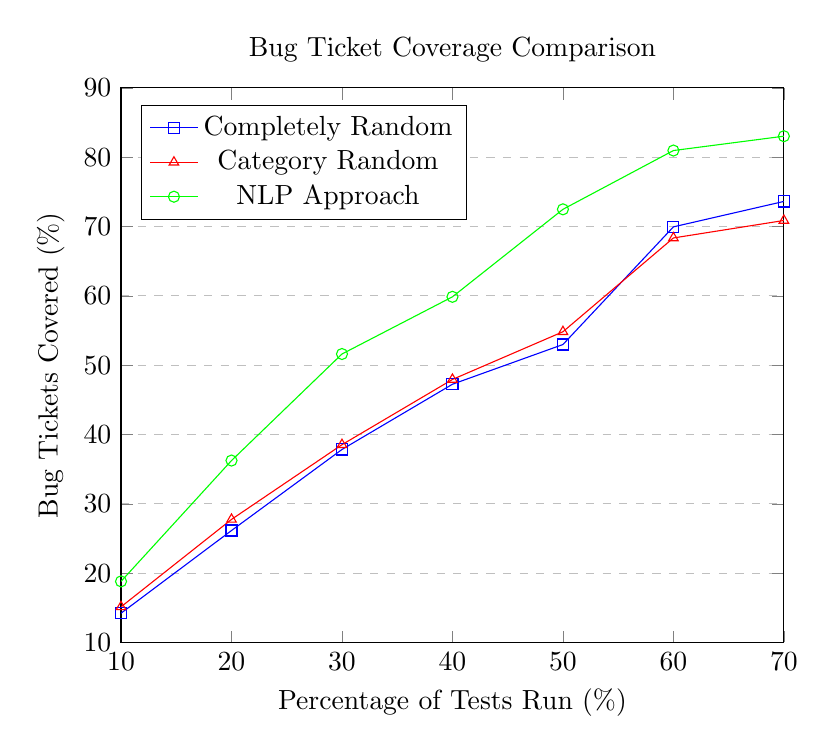
\begin{tikzpicture}
        \begin{axis}[
                title={Bug Ticket Coverage Comparison},
                xlabel={Percentage of Tests Run (\%)},
                ylabel={Bug Tickets Covered (\%)},
                xmin=10, xmax=70,
                ymin=10, ymax=90,
                xtick={10,20,30,40,50,60,70},
                ytick={10,20,30,40,50,60,70,80,90},
                legend pos=north west,
                ymajorgrids=true,
                grid style=dashed,
            ]

            \addplot[
                color=blue,
                mark=square,
            ]
            coordinates {
                    (10,14.22)(20,26.15)(30,37.84)(40,47.25)(50,52.98)(60,69.95)(70,73.62)
                };
            \addlegendentry{Completely Random}

            \addplot[
                color=red,
                mark=triangle,
            ]
            coordinates {
                    (10,15.14)(20,27.75)(30,38.53)(40,47.94)(50,54.82)(60,68.35)(70,70.87)
                };
            \addlegendentry{Category Random}

            \addplot[
                color=green,
                mark=o,
            ]
            coordinates {
                    (10,18.81)(20,36.24)(30,51.61)(40,59.86)(50,72.48)(60,80.96)(70,83.03)
                };
            \addlegendentry{NLP Approach}

        \end{axis}
    \end{tikzpicture}
    \caption{Comparison of different test selection approaches in terms of bug tickets covered.}
    \label{fig:bugticketcoverage}
\end{figure}

Table \ref{fig:bugticketcoverage} shows that a \ac{NLP}-based selection of 30\% of the tests achieves a bug detection quota of 51.61\%, while 50\% results in a quota of 72.48\%.
This means we can still detect nearly $\frac{3}{4}$ of all bugs when only executing $\frac{1}{2}$ of all tests.
We can also see that the naive approaches are very similar to each other and perform worse than the \ac{NLP}-based selection. 
For the first naive approach, Table \ref{fig:bugticketcoverage} shows that a random selection of 30\% of tests results in a bug detection quota of 37.84\%, while a selection of 30\% of tests results in 52.98\% of bug tickets covered.

The next naive approach was to select based on categories. Selecting 30\% of test cases from separate categories showed a bug detection quota of 38.53\%, while a selection of 50\% covered 54.82\% of bug tickets.
\section{Discussion}
Especially for larger percentages, clustering takes quite a substantial amount
of time -> worth it?
\section{Threats to Validity}

\subsection*{External:} 
The dataset of XWiki might not represent all manual test suites equally. It is possible that the suite was a lucky choice for our approach and other datasets might not have the same level of improvements over random selection. If the XWiki dataset has bug distributions significantly different from what is commonly seen in software projects (e.g., very few bugs concentrated in a small portion of the system), it might limit the generalizability of the findings.
Also, if the quality of test case descriptions varies significantly (level of detail, clarity etc.), it could weaken the quality of the NLP analysis and clustering.


\subsection*{Internal:} 
There might be some bugs that are more important or take more time than others. If the \ac{NLP}-based approach only selects dissimilar tests, we might have a bias on not executing a set of more important test cases if they are too similar to each other and thereby might not find a set of more important bugs.
While textual similarity of test case steps leads to an improvement of bug coverage in our case, it is not guaranteed that it actually effectively identifies test similarity all the time. Not every relation between tests might be covered by textual similarity and there might even be datasets where the textual similarity does not at all correlate with similar code that is tested in the background. This could lead to drastically worse results on other datasets.

\subsection*{Mitigation}
To avoid these threats one might want to introduce bigger datasets and also look at the severity of bugs. On top of that, manually identifying similar tests might give an idea of how good \ac{NLP}-based similarity works to find similar tests compared to other approaches and might display inadequacies of this approach.
Also, including other parts of the test case descriptions and a different way to cluster the embeddings could improve bug coverage even more and make the \ac{NLP}-based approach work on more datasets that might not work with our exact approach.

\section{Conclusion}
\label{sec:conclusion}

The results of this paper show that using NLP techniques to cluster test cases based on textual similarity offers notable improvements in bug detection efficiency compared to simpler test selection methods. Selecting even 30\% of tests using our approach revealed a substantially improved bug detection rate compared to just selecting random tests. 

As human resources might become a problem for rapidly growing projects that also have a growing number of manual tests to be performed, especially in the open-source world, our method can achieve a favorable tradeoff between time spent testing and bugs covered.

Furthermore,  our work supports the findings of Viggiato et al. \cite{Viggiato}, indicating that textual similarity of test steps provides a useful indicator of overall test case similarity, at least within our dataset.
%
% ---- Bibliography ----
%
\bibliographystyle{splncs04}
\bibliography{library.bib}
%
\end{document}
